%% bare_jrnl.tex
%% V1.4b
%% 2015/08/26
%% by Michael Shell
%% see http://www.michaelshell.org/
%% for current contact information.
%%
%% This is a skeleton file demonstrating the use of IEEEtran.cls
%% (requires IEEEtran.cls version 1.8b or later) with an IEEE
%% journal paper.
%%
%% Support sites:
%% http://www.michaelshell.org/tex/ieeetran/
%% http://www.ctan.org/pkg/ieeetran
%% and
%% http://www.ieee.org/

%%*************************************************************************
%% Legal Notice:
%% This code is offered as-is without any warranty either expressed or
%% implied; without even the implied warranty of MERCHANTABILITY or
%% FITNESS FOR A PARTICULAR PURPOSE! 
%% User assumes all risk.
%% In no event shall the IEEE or any contributor to this code be liable for
%% any damages or losses, including, but not limited to, incidental,
%% consequential, or any other damages, resulting from the use or misuse
%% of any information contained here.
%%
%% All comments are the opinions of their respective authors and are not
%% necessarily endorsed by the IEEE.
%%
%% This work is distributed under the LaTeX Project Public License (LPPL)
%% ( http://www.latex-project.org/ ) version 1.3, and may be freely used,
%% distributed and modified. A copy of the LPPL, version 1.3, is included
%% in the base LaTeX documentation of all distributions of LaTeX released
%% 2003/12/01 or later.
%% Retain all contribution notices and credits.
%% ** Modified files should be clearly indicated as such, including  **
%% ** renaming them and changing author support contact information. **
%%*************************************************************************


% *** Authors should verify (and, if needed, correct) their LaTeX system  ***
% *** with the testflow diagnostic prior to trusting their LaTeX platform ***
% *** with production work. The IEEE's font choices and paper sizes can   ***
% *** trigger bugs that do not appear when using other class files.       ***                          ***
% The testflow support page is at:
% http://www.michaelshell.org/tex/testflow/



\documentclass[journal, twoside]{IEEEtran}
%
% If IEEEtran.cls has not been installed into the LaTeX system files,
% manually specify the path to it like:
% \documentclass[journal]{../sty/IEEEtran}





% Some very useful LaTeX packages include:
% (uncomment the ones you want to load)


% *** MISC UTILITY PACKAGES ***
%
%\usepackage{ifpdf}
% Heiko Oberdiek's ifpdf.sty is very useful if you need conditional
% compilation based on whether the output is pdf or dvi.
% usage:
% \ifpdf
%   % pdf code
% \else
%   % dvi code
% \fi
% The latest version of ifpdf.sty can be obtained from:
% http://www.ctan.org/pkg/ifpdf
% Also, note that IEEEtran.cls V1.7 and later provides a builtin
% \ifCLASSINFOpdf conditional that works the same way.
% When switching from latex to pdflatex and vice-versa, the compiler may
% have to be run twice to clear warning/error messages.






% *** CITATION PACKAGES ***
%
%\usepackage{cite}
% cite.sty was written by Donald Arseneau
% V1.6 and later of IEEEtran pre-defines the format of the cite.sty package
% \cite{} output to follow that of the IEEE. Loading the cite package will
% result in citation numbers being automatically sorted and properly
% "compressed/ranged". e.g., [1], [9], [2], [7], [5], [6] without using
% cite.sty will become [1], [2], [5]--[7], [9] using cite.sty. cite.sty's
% \cite will automatically add leading space, if needed. Use cite.sty's
% noadjust option (cite.sty V3.8 and later) if you want to turn this off
% such as if a citation ever needs to be enclosed in parenthesis.
% cite.sty is already installed on most LaTeX systems. Be sure and use
% version 5.0 (2009-03-20) and later if using hyperref.sty.
% The latest version can be obtained at:
% http://www.ctan.org/pkg/cite
% The documentation is contained in the cite.sty file itself.






% *** GRAPHICS RELATED PACKAGES ***
%
\ifCLASSINFOpdf
  % \usepackage[pdftex]{graphicx}
  % declare the path(s) where your graphic files are
  % \graphicspath{{../pdf/}{../jpeg/}}
  % and their extensions so you won't have to specify these with
  % every instance of \includegraphics
  % \DeclareGraphicsExtensions{.pdf,.jpeg,.png}
\else
  % or other class option (dvipsone, dvipdf, if not using dvips). graphicx
  % will default to the driver specified in the system graphics.cfg if no
  % driver is specified.
  % \usepackage[dvips]{graphicx}
  % declare the path(s) where your graphic files are
  % \graphicspath{{../eps/}}
  % and their extensions so you won't have to specify these with
  % every instance of \includegraphics
  % \DeclareGraphicsExtensions{.eps}
\fi
% graphicx was written by David Carlisle and Sebastian Rahtz. It is
% required if you want graphics, photos, etc. graphicx.sty is already
% installed on most LaTeX systems. The latest version and documentation
% can be obtained at: 
% http://www.ctan.org/pkg/graphicx
% Another good source of documentation is "Using Imported Graphics in
% LaTeX2e" by Keith Reckdahl which can be found at:
% http://www.ctan.org/pkg/epslatex
%
% latex, and pdflatex in dvi mode, support graphics in encapsulated
% postscript (.eps) format. pdflatex in pdf mode supports graphics
% in .pdf, .jpeg, .png and .mps (metapost) formats. Users should ensure
% that all non-photo figures use a vector format (.eps, .pdf, .mps) and
% not a bitmapped formats (.jpeg, .png). The IEEE frowns on bitmapped formats
% which can result in "jaggedy"/blurry rendering of lines and letters as
% well as large increases in file sizes.
%
% You can find documentation about the pdfTeX application at:
% http://www.tug.org/applications/pdftex





% *** MATH PACKAGES ***
%
%\usepackage{amsmath}
% A popular package from the American Mathematical Society that provides
% many useful and powerful commands for dealing with mathematics.
%
% Note that the amsmath package sets \interdisplaylinepenalty to 10000
% thus preventing page breaks from occurring within multiline equations. Use:
%\interdisplaylinepenalty=2500
% after loading amsmath to restore such page breaks as IEEEtran.cls normally
% does. amsmath.sty is already installed on most LaTeX systems. The latest
% version and documentation can be obtained at:
% http://www.ctan.org/pkg/amsmath





% *** SPECIALIZED LIST PACKAGES ***
%
%\usepackage{algorithmic}
% algorithmic.sty was written by Peter Williams and Rogerio Brito.
% This package provides an algorithmic environment fo describing algorithms.
% You can use the algorithmic environment in-text or within a figure
% environment to provide for a floating algorithm. Do NOT use the algorithm
% floating environment provided by algorithm.sty (by the same authors) or
% algorithm2e.sty (by Christophe Fiorio) as the IEEE does not use dedicated
% algorithm float types and packages that provide these will not provide
% correct IEEE style captions. The latest version and documentation of
% algorithmic.sty can be obtained at:
% http://www.ctan.org/pkg/algorithms
% Also of interest may be the (relatively newer and more customizable)
% algorithmicx.sty package by Szasz Janos:
% http://www.ctan.org/pkg/algorithmicx




% *** ALIGNMENT PACKAGES ***
%
%\usepackage{array}
% Frank Mittelbach's and David Carlisle's array.sty patches and improves
% the standard LaTeX2e array and tabular environments to provide better
% appearance and additional user controls. As the default LaTeX2e table
% generation code is lacking to the point of almost being broken with
% respect to the quality of the end results, all users are strongly
% advised to use an enhanced (at the very least that provided by array.sty)
% set of table tools. array.sty is already installed on most systems. The
% latest version and documentation can be obtained at:
% http://www.ctan.org/pkg/array


% IEEEtran contains the IEEEeqnarray family of commands that can be used to
% generate multiline equations as well as matrices, tables, etc., of high
% quality.




% *** SUBFIGURE PACKAGES ***
%\ifCLASSOPTIONcompsoc
%  \usepackage[caption=false,font=normalsize,labelfont=sf,textfont=sf]{subfig}
%\else
%  \usepackage[caption=false,font=footnotesize]{subfig}
%\fi
% subfig.sty, written by Steven Douglas Cochran, is the modern replacement
% for subfigure.sty, the latter of which is no longer maintained and is
% incompatible with some LaTeX packages including fixltx2e. However,
% subfig.sty requires and automatically loads Axel Sommerfeldt's caption.sty
% which will override IEEEtran.cls' handling of captions and this will result
% in non-IEEE style figure/table captions. To prevent this problem, be sure
% and invoke subfig.sty's "caption=false" package option (available since
% subfig.sty version 1.3, 2005/06/28) as this is will preserve IEEEtran.cls
% handling of captions.
% Note that the Computer Society format requires a larger sans serif font
% than the serif footnote size font used in traditional IEEE formatting
% and thus the need to invoke different subfig.sty package options depending
% on whether compsoc mode has been enabled.
%
% The latest version and documentation of subfig.sty can be obtained at:
% http://www.ctan.org/pkg/subfig




% *** FLOAT PACKAGES ***
%
%\usepackage{fixltx2e}
% fixltx2e, the successor to the earlier fix2col.sty, was written by
% Frank Mittelbach and David Carlisle. This package corrects a few problems
% in the LaTeX2e kernel, the most notable of which is that in current
% LaTeX2e releases, the ordering of single and double column floats is not
% guaranteed to be preserved. Thus, an unpatched LaTeX2e can allow a
% single column figure to be placed prior to an earlier double column
% figure.
% Be aware that LaTeX2e kernels dated 2015 and later have fixltx2e.sty's
% corrections already built into the system in which case a warning will
% be issued if an attempt is made to load fixltx2e.sty as it is no longer
% needed.
% The latest version and documentation can be found at:
% http://www.ctan.org/pkg/fixltx2e


%\usepackage{stfloats}
% stfloats.sty was written by Sigitas Tolusis. This package gives LaTeX2e
% the ability to do double column floats at the bottom of the page as well
% as the top. (e.g., "\begin{figure*}[!b]" is not normally possible in
% LaTeX2e). It also provides a command:
%\fnbelowfloat
% to enable the placement of footnotes below bottom floats (the standard
% LaTeX2e kernel puts them above bottom floats). This is an invasive package
% which rewrites many portions of the LaTeX2e float routines. It may not work
% with other packages that modify the LaTeX2e float routines. The latest
% version and documentation can be obtained at:
% http://www.ctan.org/pkg/stfloats
% Do not use the stfloats baselinefloat ability as the IEEE does not allow
% \baselineskip to stretch. Authors submitting work to the IEEE should note
% that the IEEE rarely uses double column equations and that authors should try
% to avoid such use. Do not be tempted to use the cuted.sty or midfloat.sty
% packages (also by Sigitas Tolusis) as the IEEE does not format its papers in
% such ways.
% Do not attempt to use stfloats with fixltx2e as they are incompatible.
% Instead, use Morten Hogholm'a dblfloatfix which combines the features
% of both fixltx2e and stfloats:
%
% \usepackage{dblfloatfix}
% The latest version can be found at:
% http://www.ctan.org/pkg/dblfloatfix




%\ifCLASSOPTIONcaptionsoff
%  \usepackage[nomarkers]{endfloat}
% \let\MYoriglatexcaption\caption
% \renewcommand{\caption}[2][\relax]{\MYoriglatexcaption[#2]{#2}}
%\fi
% endfloat.sty was written by James Darrell McCauley, Jeff Goldberg and 
% Axel Sommerfeldt. This package may be useful when used in conjunction with 
% IEEEtran.cls'  captionsoff option. Some IEEE journals/societies require that
% submissions have lists of figures/tables at the end of the paper and that
% figures/tables without any captions are placed on a page by themselves at
% the end of the document. If needed, the draftcls IEEEtran class option or
% \CLASSINPUTbaselinestretch interface can be used to increase the line
% spacing as well. Be sure and use the nomarkers option of endfloat to
% prevent endfloat from "marking" where the figures would have been placed
% in the text. The two hack lines of code above are a slight modification of
% that suggested by in the endfloat docs (section 8.4.1) to ensure that
% the full captions always appear in the list of figures/tables - even if
% the user used the short optional argument of \caption[]{}.
% IEEE papers do not typically make use of \caption[]'s optional argument,
% so this should not be an issue. A similar trick can be used to disable
% captions of packages such as subfig.sty that lack options to turn off
% the subcaptions:
% For subfig.sty:
% \let\MYorigsubfloat\subfloat
% \renewcommand{\subfloat}[2][\relax]{\MYorigsubfloat[]{#2}}
% However, the above trick will not work if both optional arguments of
% the \subfloat command are used. Furthermore, there needs to be a
% description of each subfigure *somewhere* and endfloat does not add
% subfigure captions to its list of figures. Thus, the best approach is to
% avoid the use of subfigure captions (many IEEE journals avoid them anyway)
% and instead reference/explain all the subfigures within the main caption.
% The latest version of endfloat.sty and its documentation can obtained at:
% http://www.ctan.org/pkg/endfloat
%
% The IEEEtran \ifCLASSOPTIONcaptionsoff conditional can also be used
% later in the document, say, to conditionally put the References on a 
% page by themselves.




% *** PDF, URL AND HYPERLINK PACKAGES ***
%
%\usepackage{url}
% url.sty was written by Donald Arseneau. It provides better support for
% handling and breaking URLs. url.sty is already installed on most LaTeX
% systems. The latest version and documentation can be obtained at:
% http://www.ctan.org/pkg/url
% Basically, \url{my_url_here}.




% *** Do not adjust lengths that control margins, column widths, etc. ***
% *** Do not use packages that alter fonts (such as pslatex).         ***
% There should be no need to do such things with IEEEtran.cls V1.6 and later.
% (Unless specifically asked to do so by the journal or conference you plan
% to submit to, of course. )


% correct bad hyphenation here
\hyphenation{op-tical net-works semi-conduc-tor}
\usepackage{amsmath}
\usepackage[pdftex]{graphicx}
\usepackage{caption}
\usepackage{textcomp}
\usepackage[labelfont=up,labelsep=newline, font=scriptsize, skip=1ex]{caption}


%Koushik's pakages%
\usepackage{amsthm}
\usepackage[bb=boondox]{mathalfa}
\usepackage[normalem]{ulem}
\useunder{\uline}{\ul}{}


%\graphicspath{ {./Figures/} }
\begin{document}
%
% paper title
% Titles are generally capitalized except for words such as a, an, and, as,
% at, but, by, for, in, nor, of, on, or, the, to and up, which are usually
% not capitalized unless they are the first or last word of the title.
% Linebreaks \\ can be used within to get better formatting as desired.
% Do not put math or special symbols in the title.
\title{A Regression Approach to Music\\ Emotion Recognition}
%
%
% author names and IEEE memberships
% note positions of commas and nonbreaking spaces ( ~ ) LaTeX will not break
% a structure at a ~ so this keeps an author's name from being broken across
% two lines.
% use \thanks{} to gain access to the first footnote area
% a separate \thanks must be used for each paragraph as LaTeX2e's \thanks
% was not built to handle multiple paragraphs
%

\author{Yi-Hsuan~Yang,
        Yu-Ching~Lin,
        Ya-Fan~Su,
        and~Homer~H.~Chen,~\IEEEmembership{Fellow,~IEEE}% <-this % stops a space
\thanks{Manuscript received December 16, 2006; revised September 20, 2007. This
work was supported in part by grants from the National Science Council of
Taiwan under Contracts NSC 96–2219–E-003 and NSC 96–2725–E-002–PAE.
The associate editor coordinating the review of this manuscript and approving
it for publication was Dr. Dan Ellis.}% <-this % stops a space
\thanks{Y.-H. Yang, Y.-C. Lin, and Y.-F. Su are with the Graduate Institute of Com-munication Engineering, National Taiwan University, Taipei 10617, Taiwan, R.O.C. (e-mail: affige@gamil.com, vagante@gmail.com, b92901017@ntu.edu.tw).}% <-this % stops a space
\thanks{H. H. Chen is with the Graduate Institute of Communication Engineering, the Graduate Institute of Networking and Multimedia, and the Department of Elec-trical Engineering, National Taiwan University, Taipei 10617, Taiwan, R.O.C. (e-mail: homer@cc.ee.ntu.edu.tw).}
\thanks{Color versions of one or more of the figures in this paper are available online at http://ieeexplore.ieee.org.}
\thanks{Digital Object Identifier 10.1109/TASL.2007.911513}}


% note the % following the last \IEEEmembership and also \thanks - 
% these prevent an unwanted space from occurring between the last author name
% and the end of the author line. i.e., if you had this:
% 
% \author{....lastname \thanks{...} \thanks{...} }
%                     ^------------^------------^----Do not want these spaces!
%
% a space would be appended to the last name and could cause every name on that
% line to be shifted left slightly. This is one of those "LaTeX things". For
% instance, "\textbf{A} \textbf{B}" will typeset as "A B" not "AB". To get
% "AB" then you have to do: "\textbf{A}\textbf{B}"
% \thanks is no different in this regard, so shield the last } of each \thanks
% that ends a line with a % and do not let a space in before the next \thanks.
% Spaces after \IEEEmembership other than the last one are OK (and needed) as
% you are supposed to have spaces between the names. For what it is worth,
% this is a minor point as most people would not even notice if the said evil
% space somehow managed to creep in.



% The paper headers
\markboth{IEEE TRANSACTIONS ON AUDIO,~SPEECH,~AND~LANGUAGE~PROCESSING,~VOL.~16, NO.~2,~FEBRUARY~2008}
{IEEE TRANSACTIONS ON AUDIO,~SPEECH,~AND~LANGUAGE~PROCESSING,~VOL.~16, NO.~2,~FEBRUARY~2008}
\markright{YANG \MakeLowercase{\textit{et al.}}: REGRESSION APPROACH TO MUSIC EMOTION RECOGNITION}
% The only time the second header will appear is for the odd numbered pages
% after the title page when using the twoside option.
% 
% *** Note that you probably will NOT want to include the author's ***
% *** name in the headers of peer review papers.                   ***
% You can use \ifCLASSOPTIONpeerreview for conditional compilation here if
% you desire.




% If you want to put a publisher's ID mark on the page you can do it like
% this:
\IEEEpubid{1558-7916/\$25.00 \textcopyright\ 2008 IEEE}
% Remember, if you use this you must call \IEEEpubidadjcol in the second
% column for its text to clear the IEEEpubid mark.



% use for special paper notices
%\IEEEspecialpapernotice{(Invited Paper)}


\IEEEaftertitletext{\vspace{-2\baselineskip}}

% make the title area
\maketitle

% As a general rule, do not put math, special symbols or citations
% in the abstract or keywords.
\begin{abstract}
Content-based retrieval has emerged in the face of
content explosion as a promising approach to information access.
In this paper, we focus on the challenging issue of recognizing the
emotion content of music signals, or music emotion recognition
(MER). Specifically, we formulate MER as a regression problem
to predict the arousal and valence values (AV values) of each music
sample directly. Associated with the AV values, each music sample
becomes a point in the arousal-valence plane, so the users can ef-
ficiently retrieve the music sample by specifying a desired point
in the emotion plane. Because no categorical taxonomy is used,
the regression approach is free of the ambiguity inherent to conventional categorical approaches. To improve the performance, we apply principal component analysis to reduce the correlation between arousal and valence, and RReliefF to select important features. An extensive performance study is conducted to evaluate the
accuracy of the regression approach for predicting AV values. The
best performance evaluated in terms of the $R^2$ statistics reaches
58.3\% for arousal and 28.1\% for valence by employing support
vector machine as the regressor. We also apply the regression approach to detect the emotion variation within a music selection and
find the prediction accuracy superior to existing works. A group-
wise MER scheme is also developed to address the subjectivity issue
of emotion perception.
\end{abstract}

% Note that keywords are not normally used for peerreview papers.
\begin{IEEEkeywords}
Arousal, music emotion recognition (MER), re-
gression, support vector machine, valence.
\end{IEEEkeywords}






% For peer review papers, you can put extra information on the cover
% page as needed:
% \ifCLASSOPTIONpeerreview
% \begin{center} \bfseries EDICS Category: 3-BBND \end{center}
% \fi
%
% For peerreview papers, this IEEEtran command inserts a page break and
% creates the second title. It will be ignored for other modes.
\IEEEpeerreviewmaketitle



\section{Introduction}
% The very first letter is a 2 line initial drop letter followed
% by the rest of the first word in caps.
% 
% form to use if the first word consists of a single letter:
% \IEEEPARstart{A}{demo} file is ....
% 
% form to use if you need the single drop letter followed by
% normal text (unknown if ever used by the IEEE):
% \IEEEPARstart{A}{}demo file is ....
% 
% Some journals put the first two words in caps:
% \IEEEPARstart{T}{his demo} file is ....
% 
% Here we have the typical use of a "T" for an initial drop letter
% and "HIS" in caps to complete the first word.
\IEEEPARstart{M}{USIC} plays an important role in human\textquotesingle s history, even more so in the digital age. Never before has such a large
collection of music been created and accessed daily by people.
As the amount of content continues to explode, the way music
information is organized has to evolve in order to meet the ever
increasing demand for easy and effective information access.
Music classification and retrieval by emotion is a plausible ap-
proach, for it is content-centric and functionally powerful. 

\begin{figure}[h]
\centering
\captionsetup{justification=centering}
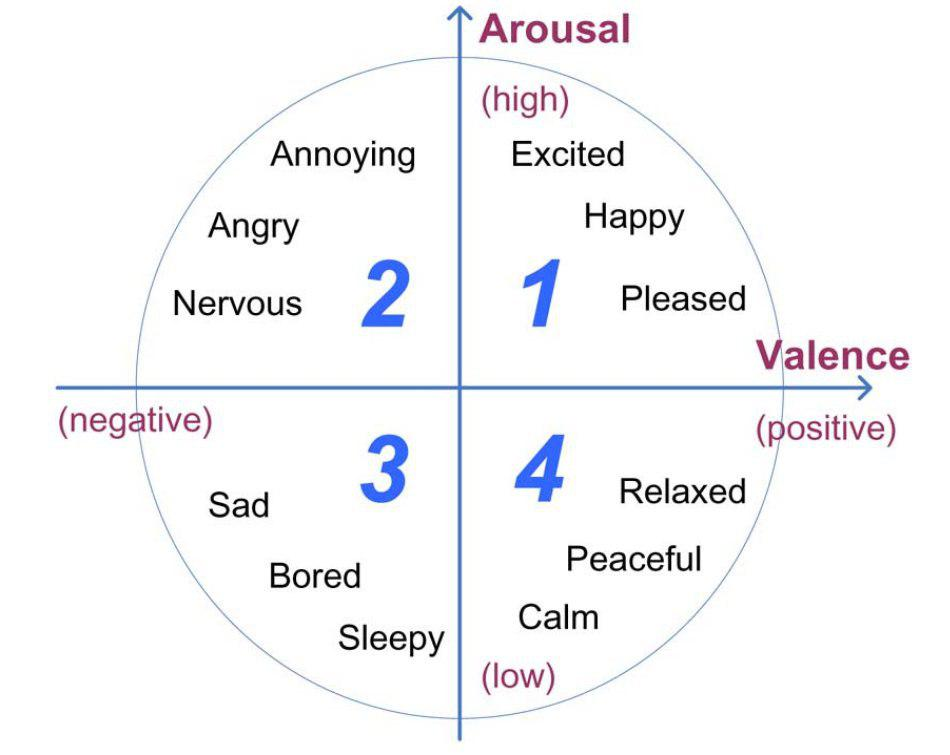
\includegraphics[width=0.4\textwidth, height=0.3\textwidth]{fig1.png}
\caption{Thayer’s arousal-valence emotion plane.}
\label{fig1}
\end{figure}

Emotion recognition from music signal is a challenging task
due to the following reasons. First, emotion perception is intrinsically subjective, and people can perceive different emotions for the same song. This subjectivity issue makes the performance evaluation of an MER system fundamentally difficult because a common agreement on the classification result is hard to
obtain. Second, it is not easy to describe emotion in a universal
way because the adjectives used to describe emotions may be
ambiguous, and the use of adjectives for the same emotion can
vary from person to person. Third, it is still inexplicable how
music evokes emotion. What intrinsic element of music, if any,
creates a specific emotional response in the listener is still far
from well-understood.

To uncover the relationship between music and emotion,
many previous works \cite{1}--\cite{8} have categorized emotions into
a number of emotion classes and applied the standard pattern
recognition procedure to train a classifier. The methods de-
scribed in \cite{1} and \cite{2} adopt the basic emotions such as happy,
angry, sad, and fear as the emotion classes, whereas the methods
described in \cite{3}--\cite{8} recognize the ambiguity of adjectives and
define the emotion classes in terms of arousal (how exciting or
calming) and valence (how positive or negative). For example,
the emotion classes can be divided into the four quadrants in
Thayer’s arousal-valence emotion plane \cite{12}, Fig. 1.

However, even with the emotion plane, the categorical tax-
onomy of emotion classes is still inherently ambiguous. Each
emotion class represents an area in the emotion plane, and the
emotion states within each area may vary a lot. For example,
the first quadrant of the emotion plan contains emotions such as
excited, happy, and pleased, which are different in nature. This
ambiguity confuses the subjects in the subjective test and con-
fuses the users when retrieving a music piece according to their
emotion states.% You must have at least 2 lines in the paragraph with the drop letter
% (should never be an issue)



\IEEEpubidadjcol
An alternative is to view the emotion plane as a continuous
space and recognize each point of the plane as an emotion state.
In this way, the ambiguity associated with emotion classes or ad-
jectives can be successfully avoided since no categorical classes
are needed. This continuous perspective has been adopted by
psychologists to model the emotional response of the subjects
\cite{13}, \cite{14}. In \cite{15}, the software “FEELTRACE” is developed
to let subjects track the emotion content of a stimulus (such as
speech, music, or video) as they perceive it over time. However,
a major issue of the continuous perspective is that arousal and
valence are not necessarily independent and can in fact impact
each other. Whether the emotion states should be modeled as
categories or continua has been a debate in psychology, and ei-
ther perspective has its pros and cons. For MER, the continuous
perspective is considered more appropriate since it resolves the
ambiguity issue.
\IEEEpubidadjcol

Specifically, with the continuous approach, we first compute
the arousal and valence values (AV values) of each music sample
and view the music sample as a point in the emotion plane. Then
the user can retrieve music by specifying a point in the emotion
plane according to his/her emotion state, and the system would
return the music pieces whose locations are closest to the spec-
ified point. In this way, apparently, the efficiency and accuracy
of music retrieval is much improved.

The viability of the continuous approach heavily lies in the
prediction accuracy of the AV values. Since automatic calcula-
tion of the AV values (AV computation) is still at its early stage,
and the performance of existing approaches \cite{8}–-\cite{11} is unsatis-
factory in many aspects (see Section II), a primary task of this
paper is to develop an effective method for AV computation. We
propose to formulate MER as a regression problem and use re-
gression techniques to directly predict the AV values of music
samples from the extracted features. This computational algo-
rithm has sound theoretical basis, allows thorough performance
study, and generally exhibits reliable prediction performance.
The other main issue, the dependency between arousal and va-
lence, is addressed by reducing the data correlation by principal
component analysis \cite{16}.

An extensive performance study is conducted to evaluate the
prediction accuracy of the proposed regression approach by
using different combination of data spaces, feature spaces, and
regression algorithms. Support vector regression \cite{18} is found
to produce better prediction accuracy than linear regression
\cite{17} and AdaBoost.RT \cite{20}. The $R^2$
statistics \cite{17} reaches
58.3\% for arousal and 28.1\% for valence. Because there are
no other existing systems viewing MER from a continuous
perspective, we apply the regression approach to detect the
emotion variation within music selections and find it is superior
to the one proposed in \cite{10}.

In summary, the primary contributions of the paper include
the following.
\vspace{-0.5em}
\begin{itemize}
    \item To the best of our knowledge, this work represents one of the first attempts that develop an MER system from a continuous perspective and represent each song as a point in the emotion plane. This approach is free of the ambiguity issue of MER.
    \begin{table}[ht]
    \centering
        \caption{COMPARISON OF WORKS ON MUSIC EMOTION}
        \label{table1}
    \begin{tabular}{ccl}
    \hline
    Field                 & Perspective & \multicolumn{1}{c}{Description}                                                                               \\ \hline
    MER {[}1{]}-{[}8{]}   & categorical & \begin{tabular}[c]{@{}l@{}}Classifying music selections into\\ several classes based on emotion.\end{tabular} \\ \hline
    MEVD {[}8{]}-{[}11{]} & continuous  & \begin{tabular}[c]{@{}l@{}}Detecting the emotion variation\\ within a music selection.\end{tabular}           \\ \hline
    MER(this work)        & continuous  & \begin{tabular}[c]{@{}l@{}}Representing each music selection\\ as a point in the emotion plane.\end{tabular}  \\ \hline
    \end{tabular}
    \end{table}
    \item A novel AV computation method based on the regression theory is proposed. Principal component analysis \cite{16} is employed to reduce the data correlation, and RReliefF \cite{22} is utilized for feature selection (Sections III and IV).
    \item An extensive performance study is conducted to demonstrate the accuracy and effectiveness of the regression approach for both music emotion recognition and music emotion variation detection (Section V).
    \item A group-wise MER scheme is proposed to solve the subjectivity issue of MER (Section VI).
\end{itemize}
%\hfill mds
%\hfill August 26, 2015
\section{RELATED WORKS}
Despite a great deal of effort that has been made for MER in
recent years \cite{1}--\cite{8}, little attention has been paid to view the
emotion plane from a continuous perspective. Some exceptions
can be found in the music emotion variation detection (MEVD)
field \cite{8}--\cite{11}, where the emotion content of music is quantified as a time-varying continuous variable, and some statistical
methods are developed to predict the emotion variation. How-
ever, detecting the emotion variation is different from representing each song individually as a point in the emotion plane.
Our work represents one of the first attempts pioneering this
novel perspective. See Table I for a comparison.

In the following, we give brief review of existing AV computation methods and illuminate the rational of adopting the regression approach rather than these methods.

\subsection{Arousal and Valence Modeling (AV Modeling)}
To detect the emotion variation in video sequences, AV modeling is proposed in \cite{9} to compute the AV values. The arousal and valence models are weighted combinations of some component functions that are computed along the timeline. The resulting arousal and valence curves are combined to form an effective curve, making it easy to trace the emotion variation of video content and to identify the segments with high emotional
content. The component functions used for arousal are the motion vectors between consecutive video frames, the changes in shot lengths, and the energy of sound. Valence is modeled by the pitch of sound.

Although AV modeling is based on some psychological understandings and the adopted features are intuitively related to emotion perception, it is difficult to evaluate the performance quantitatively due to lack of theoretical foundation. A rigorous approach that allows performance study is more favorable. Furthermore, unlike video, there are fewer salient music features that have strong link to emotion perception.
\subsection{Fuzzy Approach}
\begin{table}[ht]
    \centering
        \caption{COMPARISON OF THE EXISTING METHODS FOR AV COMPUTATION}
        \label{table2}

    \begin{tabular}{ccccc}
    \hline
    Name                & Field & Accuracy                                                        & \begin{tabular}[c]{@{}c@{}}Temporal\\ information\end{tabular} & \begin{tabular}[c]{@{}c@{}}Geometric\\ operation\end{tabular} \\ \hline
    AV modeling {[}9{]} & Video & N/A                                                             & No need                                                        & No need                                                       \\ \hline
    Fuzzy{[}8{]}        & Music & N/A                                                             & No need                                                        & Need                                                          \\ \hline
    System ID {[}10{]}  & Music & \begin{tabular}[c]{@{}c@{}}78.4\% (a)\\ 21.9\% (v)\end{tabular} & Need                                                           & No need                                                       \\ \hline
    \end{tabular}
\end{table}
In \cite{8}, emotion classes are divided into four quadrants in the emotion plane (see Fig. 1), and each input sample is assigned a fuzzy vector indicating the relative strength of each class by fuzzy classifiers \cite{24}, \cite{25}. For example, a fuzzy vector of four emotion classes is expressed as
\begin{equation}
\mu =  \left\{ \mu_1,\mu_2,\mu_3,\mu_4 \right\},    \sum_{i=1}^4\mu_i=1 
\end{equation}
where $\mu_i\geq 0$ is the relative strength of class $i$. The final decision
of classification is the class with the maximal strength.

Given a fuzzy vector, the fuzzy approach exploits the geometric relationship of the four emotion classes and computes the AV values by the following transformation:
\begin{equation}
    a = \mu_1+\mu_2-\mu_3-\mu4
\end{equation}
\begin{equation}
    v = \mu_1+\mu_4-\mu_2-\mu3
\end{equation}
where $a$ denotes arousal and $v$ denotes valence. However, the transformation involves emotion classes that are not necessarily independent of, and orthogonal to, each other. Since the geometric relationship between arousal and valence is inexact, it is improper to perform arithmetic operations on the AV values. Besides, similar to AV modeling, the fuzzy approach is short of a quantitative performance evaluation mechanism for lack of ground truth.
\vspace{-1em}
\subsection{System Identification Approach (System ID)}
A systematic approach for MEVD is proposed in \cite{10},
where the system identification technique is utilized to model
the music emotion as a function of 18 musical features. The
ground truth data are collected every second, so the music
selections are also segmented every second before feature
extraction is performed. Six western classical music selections
of various moods form the dataset. Results demonstrate that
system identification provides a means to the generalization of
the emotional content for a genre of music (western classical music), and the reported average $R^2$ statistics \cite{17} is 78.4\% for arousal and 21.9\% for valence.

However, the system ID approach, as well as the time series
analysis approach proposed earlier by Schubert \cite{11}, computes
the AV values by exploiting the temporal relationship between
music segments, which is absent for MER.

A comparison of the reviewed methods in terms of the ability
to compute the AV values is summarized in Table II. To sum up,
a robust AV computation algorithm should have a sound theoretical foundation and allows quantitative performance study.
Among the reviewed methods, only the system ID approach embeds a theoretical structure, yet it utilizes the temporal information which is not available for MER. In addition, the computation of AV values should be made without applying any geometric operation between arousal and valence due to their inexact relationship. It is also favorable to have the computation algorithm directly predict real values (i.e., arousal or valence)
from extracted features.


\section{REGRESSION APPROACH}
Regression theory is a well-studied theory aiming at predicting a real value from observed variables (or features). It
has a sound theoretical foundation, allows easy performance
analysis and optimization, and generally provides reliable
prediction performance \cite{17}. Besides, no temporal information
or geometric operation is needed. Therefore, formulating MER
as a regression problem seems to be a promising approach.
Below, we first describe how the formulation is made, then
present the system description in detail. The performance study
of the regression approach is reported in Section V.

    Given \( N \) inputs , \((x_i,y_i), 1\leq i\leq N\) , where \(x_i\) is a feature
vector for the \(i_{th}\) input sample, and \(y_i \in \mathbb{R}\) (\(\mathbb{R}\) denotes a set of real values) is the real value to be predicted for the \(i\)th sample,
the regression system trains a regression algorithm (regressor) \(R(.)\) such that the mean squared error \(\varepsilon\) is minimized [17]:
\begin{equation}
\varepsilon = \frac{1}{N} \sum_{i=1}^{N} (y_i - R(x_i))^2
\end{equation}
where\(R(x_i)\) is the prediction result for the \(i\)th sample.

Since the AV values are viewed upon as real values from the
continuous perspective, the regression theory can be well applied to directly predict arousal and valence. To formulate MER as a regression problem, the following considerations are taken into account.
\begin{enumerate}
    \item Domain of \(\mathbb{R}\): The Thayer’s emotion plane is viewed as a coordinate space spanned by arousal and valence, where each value is confined within \([-1,1]\).
    
    \item Ground truth: The ground truth is set via a subjective test by averaging the subjects’ opinions about the AV values of each music sample (see Section IV-C).
    
    \item Feature extraction: The extracted features need to be relevant to emotion perception for the regressor to be accurate (see Sections IV-B and V).
    
    \item Regression algorithm: Although regression theory has been well studied and many good regressors are readily available \cite{17}, the performance of a regressor is case dependent. A number of regressors should be adopted and compared to find the best one (see Section IV-D).
    
    \item Number of regressors: Since we want to predict both arousal and valence, two regressors are required and are referred to as \(R_A\) and \(R_V\).
    
    \item Training fashion: As mentioned in Section I, there is a certain degree of dependency between arousal and valence. Therefore, apart from training \(R_A\) and \(R_V\) solely independently, we need to study whether the prediction accuracy is improved if the dependency of the AV values is considered (see Section V-B).
    
\end{enumerate}

\section{SYSTEM DESCRIPTION}
Our MER system represents each music selection as a point
in the emotion plane and provides a friendly user interface for music retrieval and management. The system diagram is shown in Fig. 2, and the details are described below.

\begin{figure}[h]
\centering
\captionsetup{justification=centering}
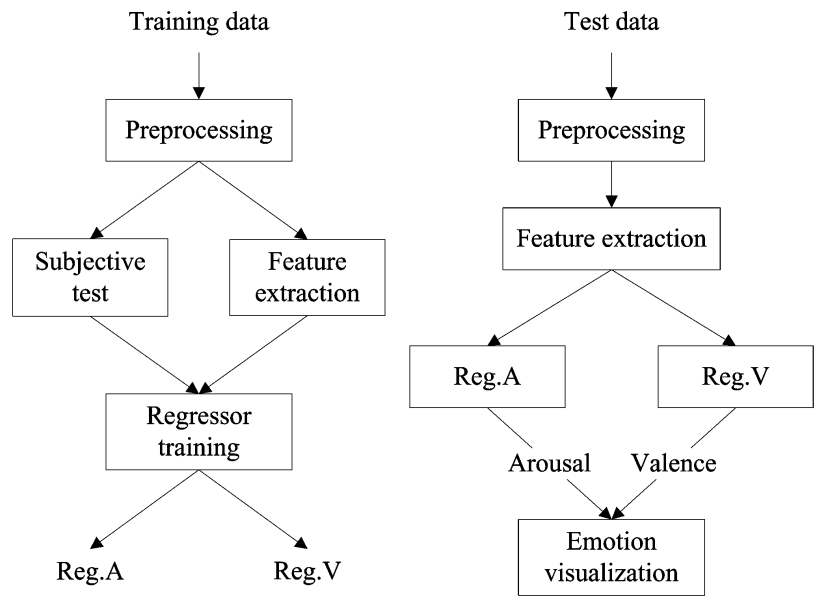
\includegraphics[width=0.4\textwidth, height=0.3\textwidth]{fig2.png}
\caption{System diagram of the proposed regression approach. Left: training phase; right: testing phase. \(R_A\) denotes the regressor for arousal, and \(R_V\) denotes the regressor for valence.}
\label{fig2}
\end{figure}

\subsection{Data Collection and Preprocessing}
The music database is made up of 195 popular songs selected from a number of Western, Chinese, and Japanese albums \cite{8}.Two criteria are used in the selection: 1) These songs should be distributed uniformly in each quadrant of the emotion plane. 2) Each music sample should express a certain dominant emotion.

Note the genre of our database is popular music of different countries rather than the western classical music, which is commonly adopted in previous works \cite{2}--\cite{5}, \cite{10}, \cite{11}. Western classical music is often chosen because it is much easier to gain agreement on perceived emotion and thus has less subjectivity issue \cite{3}. However, since the purpose of MER is to facilitate music retrieval and management in everyday music listening,
and since it is the popular music that dominates the everyday music listening, we should not shy away from the subjectivity issue by using only western classical music. More discussions
on the subjectivity issue are provided in Section VI.

To compare the segments fairly, the music samples are converted to a uniform format (22 050 Hz, 16 bits, and mono channel PCM WAV) and normalized to the same volume level. Besides, since the emotion within a music selection can vary over time \cite{8}--\cite{11}, for each song we manually select a 25-s segment (mostly the chorus part) that is representative of the
song and expresses a certain dominant emotion. Accordingly, we predict the emotion of a music segment, and regard the prediction result as the emotion of the entire song. Note we choose to trim music manually since the performance of existing music thumbnailing algorithms \cite{26} are considered not robust enough.


\subsection{Feature Extraction}
After preprocessing, we use the spectral contrast algorithm \cite{3}, DWCH algorithm \cite{2}, and two computer programs PsySound \cite{27} and Marsyas \cite{29} to extract musical features and construct a 114-dimension feature space, which is referred to as ALL hereafter. The extracted features, which are described in detail below, have been used for MER in pervious works. See Table III for denotations and brief descriptions.

\bgroup
\def\arraystretch{1.3}
\vspace{1cm}
\begin{table}[ht]
    \centering
        \caption{ADOPTED FEATURE EXTRACTION ALGORITHMS}
        \label{table3}
    
    \begin{tabular}{ccl}
\hline
Method                                                                     & \begin{tabular}[c]{@{}c@{}}Number of\\ fearure\end{tabular} & \multicolumn{1}{c}{Description}                                                                                                                                             \\ \hline
\begin{tabular}[c]{@{}c@{}}PsySound {[}27{]}\\ (P)\end{tabular}            & 44                                                          & \begin{tabular}[c]{@{}l@{}}Extracts features including loudness, level,\\ pitch multiplicity, and dissonance based on\\ psychoacoustic models.\end{tabular}                 \\ \hline
\begin{tabular}[c]{@{}c@{}}Marsyas {[}29{]}\\ (M)\end{tabular}             & 30                                                          & \begin{tabular}[c]{@{}l@{}}Extracts timbral texture, rhythmic content and \\ pitch content features. It has been shown\\ useful in music genre classification.\end{tabular} \\ \hline
\begin{tabular}[c]{@{}c@{}}Spectral\\ contrast {[}3{]}\\ (SC)\end{tabular} & 12                                                          & \begin{tabular}[c]{@{}l@{}}Represents the relative characteristics of each\\ spectral subband, and reflects the distribution\\ of harmonic components.\end{tabular}         \\ \hline
\begin{tabular}[c]{@{}c@{}}DWCH {[}2{]}\\ (D)\end{tabular}                 & 28                                                          & \begin{tabular}[c]{@{}l@{}}Daubechies wavelets coefficient histogram,\\ which has better ability in representig both \\ local and global information.\end{tabular}          \\ \hline
Total (ALL)                                                                & 144                                                         &                                                                                                                                                                             \\ \hline
\end{tabular}
    
\end{table}


\vspace{.5cm}
\begin{table}[ht]
    \centering
        \caption{15 PSYSOUND FEATURES (PSY15) RECOMMENDED IN \cite{8}}
        \label{table3}
    
    \begin{tabular}{cll}
\hline
\multicolumn{1}{l}{} & Feature             & Description                                \\ \hline
1                    & Spectral Centroid   & The centroid of spectral density function. \\
2                    & Loudness            & Human perception of sound intensity.       \\
3, 4\(^1\)            & Sharpness           & A pitchlike (low-high) aspect of timbre.   \\
5                    & Timbral Width       & The flatness of a loudness function.       \\
6                    & Volume              & Human perception of the size of the sound. \\
7, 8\(^1\)          & Spectral Dissonance & Roughness of all spectrum components.      \\
9, 10\(^1\)         & Tonal Dissonance    & Roughness of just the tonal components.    \\
11                   & Pure Tonal          & The audibility of the spectral pitches.    \\
12                   & Complex Tonal       & The audibility of the virtual pitches.     \\
13                   & Multiplicity        & The number of the pitches heard.           \\
14                   & Tonality            & major-minor tonality, e.g., A major.       \\
15                   & Chord               & Musical pitches sounded simultaneously. \\
\hline \hline
 & & \(^1\)Two algorithms used to extract the feature.
\end{tabular}
    
\end{table}
\egroup

As the name indicates, PsySound aims to model parameters of auditory sensation based on some psychoacoustic models \cite{27},\cite{28}. Four types of measures are output by PsySound: loudness, level, dissonance, and pitch. Loudness measures include loudness, sharpness (sound brightness), and timbral width (sound flatness). Level measures include sound pressure level, background noise level etc. Dissonance measures are related to the perception of short irregularities in a sound; any note in music that does not fall within the prevailing harmony is considered dissonant. Pitch measures are related to the perceived fundamental frequency of a sound  Because of this psychoacoustical foundation, the features extracted by PsySound have been found much related to emotion perception, especially 15 of them \cite{8}. Therefore, we utilize these 15 features to form a second feature space called Psy15. See Table IV for the description of Psy15.

Marsyas is a free software framework for rapid development and evaluation of computer audition applications [\cite{29}. It generates 19 timbral texture features[spectralcentroid,spectralrolloff, spectral flux, time domain zero-crossing and Mel-frequency cepstral coefficient (MFCC)], six rhythmic content features (by beat and tempo detection) and five pitch content features (by multipitch detection). Spectral centroid, spectral rolloff, and spectral flux describe spectral shape properties, zero-crossing measures the noisiness of the signal, and MFCC is a nonmusical pitch scale commonly used in speech and audio signal processing.

Spectral contrast features capture the relative spectral information in each subband and utilize the spectral peak, spectral valley, and their dynamics as features \cite{3}. The spectral contrast features also roughly reflect the relative distribution of the harmonic and nonharmonic components in the spectrum.

The Daubechies wavelets coefficient histogram (DWCH) features are computed from histograms of Daubechies wavelet coefficients at different frequency subbands with different resolutions. As \cite{2} states, due to the use of wavelet technique, DWCH features have better ability in representing both local and global information than traditional features.

PsySound and Marsyas are available online \cite{27}, \cite{29}, whereas spectral contrast and DWCH can be easily implemented in Matlab. Default values of the parameters as described in the original papers are adopted. Specifically, the analysis window for frame-level features is 23 ms (512 samples at 22 050-Hz sampling rate), and the frame-level features are
integrated to clip-level features by the MeanVar model \cite{30}, which models each frame-level feature as a Gaussian distribution and represents the feature by mean and variance. All features are linearly normalized to [0, 1].

\subsection{Subjective Test}
The subjective test sets the ground truth of the AV values. 253 volunteers are recruited from the campus. Each of them is asked to listen to ten music samples randomly drawn from the aforementioned music database and to label the AV values from –1.0 to 1.0 in 11 ordinal levels. The ground truth is set by averaging the opinions of all subjects. On average, each music sample is labeled by more than ten subjects.

Note that the subjects are asked to label the emotion based on their feelings of what the music sample is trying to evoke, rather than the emotion the subjects perceive at the test. We must make this distinction clear because perceived emotion and evoking emotion are not always the same. For example, a person who enjoys sorrowful tone might feel pleased when listening to sorrowful songs. Since MER is developed to help people retrieve music samples through a coordinate in the emotion plane, it is more natural and adequate that the AV values of a song are correspondent with the evoking emotion.

No limitations on the background (e.g., psychology expertise, musicianship, etc.) are imposed when recruiting subjects since the MER system is expected to be applicable to every common people. However, because music emotion recognition is still new to all subjects, we need to inform them the essence of the emotion model, the purpose of the experiment, and the
following rules of the subjective test.
\begin{enumerate}
    \item Label the evoking emotion rather than the perceived one.
    \item Express the general feelings in response to melody, lyrics, and singing (vocal) of the song. We do not attempt to ignore the influences of the lyrics and singing even though the related features are not considered so far.
    \item No limitation is given to the total duration of the labeling process. The subjects are allowed to listen to the music samples more than once to ensure the labels can truly reflect their feelings (typically the total duration of the labeling process is less than 15 min).
    \item Music emotion perception is in nature subjective. The subjects are free to annotate personal feeling.
\end{enumerate}

The quality of the ground truth is central to the system performance. An evaluation of the consistency of the ground truth
data is described in Section V-A.

\subsection{Regressor Training}
The 195 \((x_i,y_i)\) inputs from feature extraction and subjective test are then used to train the following three regression algorithms: multiple linear regression (MLR) \cite{17}, support vector regression (SVR)[18], and AdaBoost.RT (BoostR) \cite{20}.

MLR is a standard regression algorithm which assumes a linear relationship between variables and estimates the linear relationship by a least squares estimator. We treat MLR as the baseline approach for its simplicity.

Comparatively, SVR nonlinearly maps input feature vectors to a higher dimensional feature space by the kernel trick and yields prediction functions that are expanded on a subset of support vectors [18]. As its name indicates, SVR is an extension of the famous support vector classification, which has been found in many cases superior to existing machine learning methods. A number of previous works have adopted support vector classification for MER and reported excellent classification performance \cite{9}, \cite{4}, \cite{6}.

BoostR is another nonlinear regression algorithm in which a number of regression trees are trained iteratively and weighted according to the prediction accuracy. After the iterative process, the prediction result of each regression tree is combined (weighted mean) to form the final hypothesis. The basic underlining concept of the boosting process is based on the observation that finding a number of weak predicting rules is much easier than finding a single, highly accurate one \cite{20}. Boosting algorithms, which are the state-of-the-art methods for face detection \cite{21}, have been successfully applied in many
machine learning problems.

\subsection{Emotion Visualization}
Associated with the AV values, each music sample is visualized as a point in the emotion plane, and the similarity between music samples can be estimated by computing the Euclidean distance in the emotion plane. A user interface that supports music retrieval/recommendation by specifying a point in the emotion plane can be realized without further labeling the unseen music samples (different from that of Musicovery \cite{31}).Such a user interface can be of great use in managing large-scale music databases.

\section{PERFORMANCE STUDY}
We run a series of experiments to evaluate the performance of the regression approach. Different ground truth data spaces, feature spaces, and regression algorithms are compared in terms
\begin{figure}[h]
\centering
\captionsetup{justification=centering}
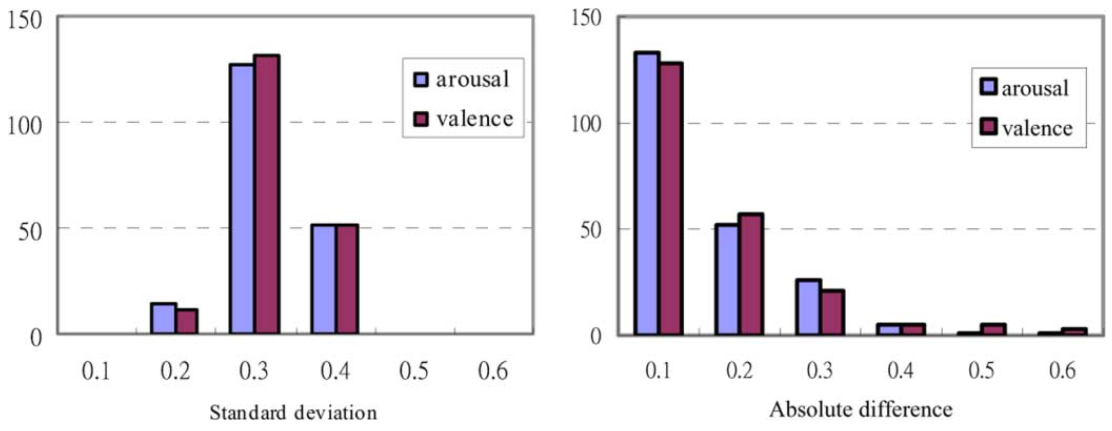
\includegraphics[width=0.48\textwidth, height=0.18\textwidth]{fig3.png}
\caption{(a) Histogram of standard deviations for arousal and valence of 195
songs in the first course of subjective test. (b) Histogram of absolute difference
for arousal and valence of 220 data pairs in the test–retest reliability study.}
\label{fig3}
\end{figure}
of the \(R^2\) statistics, which is a standard way for measuring the
goodness of fit for regression models [17]
\begin{equation}
R^2 = 1 - \frac{N \varepsilon}{ \sum_{i=1}^N (y_i - \overline{y})^2}
\end{equation}
where \(\overline{y}\) is the mean of the ground truth, and the normalization of the total squared error \((N \varepsilon)\) by the energy of the ground truth makes \(R^2\) comparable between experiments. \(R^2\) is often interpreted as the proportion of underlying data variation that is explained by the fitted regression model \cite{32}. An \(R^2\) of 1.0 means the model perfectly fits the data, while a negative \(R^2\) means the model is even worse than simply taking the sample mean. However, the kind of the \(R^2\) statistics that is satisfactory is case-dependent.

We evaluate the performance of regression by the tenfold cross validation technique \cite{16}, in which the whole dataset is randomly divided into ten parts, nine of them for training and the remaining one for testing. The above process is repeated 20 times before we compute the average result. \(R^2\) for each data dimension (say, arousal, and valence) is computed separately.

\subsection{Consistency Evaluation of the Ground Truth}
We evaluate the consistency of the ground truth in two ways. First, the consistency of annotations given by different subjects for the same song is evaluated by the standard deviation of annotations. Since the ground truth is obtained by averaging subjects’ annotations, the larger the standard deviation is, the less representative the ground truth can be.

Fig. 3(a) shows the histogram of standard deviations for arousal and valence in the first course of the subjective test. We can see that most standard deviations of music samples are about 0.3, which give rise to a 95\% confidence interval \cite{32} of roughly \(\pm{0.2}\) (sample size is ten since each music sample is labeled by more than ten subjects). On a range of \(-1.0\) to 1.0, a range of 0.4 is not that big, yet it reflects the subjectivity issue
mentioned in Section I.

Second, we evaluate whether the annotations given by the same subject are similar after a span of time by conducting a test-retest reliability study \cite{33} and computing the absolute difference between corresponding annotations for the same song. The larger the absolute difference is, the less repeatable the subjective test could be. We conduct a second course of subjective test two months after the first one, and invite 22 subjects to label the music samples they labeled in the first course again.

Fig. 3(b) shows the histogram of absolute difference for arousal and valence of 220 (22 \(\times\) 10) data pairs in the test-retest stability study. We can see that more than one half of the absolute differences fall below 0.1, showing the annotations given by the same person are quite similar.

In summary, while Fig. 3(b) shows that the subjective test by the same person is repeatable, Fig. 3(a) shows a certain degree of inconsistency in the ground truth data. The inconsistency is reasonable because music perception is subjective in nature. However, it should be noted that the consistency can be improved if we personalize the MER system, or, in a similar sense, reduce the individual differences of the subjects by grouping them according to individual factors. See Section VI for more discussions.

Using the absolute difference of test-retest reliability, we can compute an upper bound of \(R^2\) for the regression approach: 80.5\% for arousal and 58.6\% for valence. This approximated upper bound defines both the viability of the regression approach and the kind of \(R^2\) that is reasonable for the regression approach. The low upper bound for valence is not surprising since, as \cite{11} and many previous works on MER have pointed out, generally arousal is much easier to model than valence. There are two main reasons, which are actually related to each other, for this phenomenon. First, while there are a number of features relevant to arousal such as loudness (loud/soft), tempo (fast/slow), and pitch (high/low), there are few salient features for valence. Second, the perception of valence is more subjective than that of arousal; there is a good chance that people perceive opposite valence for the same song.

\subsection{Data Space}
As mentioned in Section I, a major issue of the continuous
perspective is the dependency between the two dimensions
arousal \((a)\) and valence \((v)\) in the arousal-valence (denoted as
AV) data space. The Pearson’s linear correlation coefficient
between and in our dataset can reach 0.3368; therefore, it is
interesting to see whether the performance of regression can be
improved by reducing the data correlation first.

A common method for reducing the correlation between variables is the principal component analysis (PCA)\cite{16}, which entails the computation of a loading matrix \(L\) to transform original data \(Y\) to principal components \(U\) such that
\begin{equation}
    U = L(Y - mean(Y))
\end{equation}
\begin{equation}
    Y=L^{-1}U + mean(Y)
\end{equation}
where \(U\) is the representation of \(Y\) in the principal component
space. By PCA, we are able to transform the original data space
AV to the principal component space (denoted as PC) where the
correlation between the two resulting dimensions is reduced to
nearly zero. Therefore, besides training \(R_V\) and \(R_A\), we train
another two regressors \(R_p\) and \(R_q\) in the PC space (where \(p\)
and \(q\) denote the two dimensions of PC), and then transform the
data space of the prediction results back to AV by (7). Though \(R_p\)
and \(R_q\) are also trained independently as \(R_V\) and \(R_A\), the
underlying dimensions \(p\) and \(q\) are nearly uncorrelated.

\vspace{1cm}
\bgroup
\def\arraystretch{1.3}
\begin{table}[ht]
    \centering
        \caption{FEATURE SPACES USED IN THE PERFORMANCE STUDY}
        \label{table3}
    
    \begin{tabular}{lll}
\hline
\multicolumn{1}{c}{Name} & \multicolumn{1}{c}{Dimension}                                  & \multicolumn{1}{c}{Description}                                                                                          \\ \hline
ALL                      & 114 / 114                                                      & Use the feature s in Table III.                                                                                          \\ \hline
Psy15                    & 15 / 15                                                        & Use the features in Table IV.                                                                                            \\ \hline
RRF$_{m,n}$                      & \begin{tabular}[c]{@{}l@{}}AV: 8 / 3\\ PC: 18 /15\end{tabular} & \begin{tabular}[c]{@{}l@{}}Features selected from ALL by RReliefF,\\ the dimension is selected to minimize \(\varepsilon\).\end{tabular} \\ \hline
\end{tabular}
    
\end{table}
\egroup

\subsection{Feature Space}
From the machine learning point of view, features are not necessarily of equal importance or quality, and irrelevant or redundant features may lead to inaccurate conclusion. Although domain knowledge helps identify good features, there is only limited understanding of how music evokes emotion. One solution for addressing this problem is to extract a number of musical features and then use a feature selection algorithm (FSA) to identify good features \cite{23}.

The purpose of FSA is to find the optimal feature subset that gives the maximal prediction accuracy and keeps the feature dimension minimal. For its simplicity and effectiveness, RReliefF [22] is adopted in our work. It evaluates the features one by one and assigns a real number to each feature to indicate its importance. Because RReliefF takes feature interrelationship into account, it is better than other statistical measures such as correlation coefficient, information gain, and signal to noise ratio \cite{22}.

We run RReliefF for each data space and rank the features
by importance. Then we run SVR with the top-$m$ and top-$n$ selected features for the two dimensions in each data space to
decide the best combination of $m$ and $n$ that lead to minimal $\varepsilon$. The top-$m$ and top-$n$ selected features form the third feature space RRF$_{m,n}$ . The best feature dimensions $m$ and $n$ of
RRF, along with the adopted feature spaces, are summarized in
Table V. We show the comparison of using different feature dimensions for AV and PC in Fig. 4, and list the top five RRF features for AV in Table VI. From Table VI, we can see that the top
features for arousal are related to spectral shape and pitch, and
the top features for valence are more related to rhythmic (beat
and tempo) and pitch properties of sound. Note for valence, the
combination of the first three features gives rise to the minimal
mean squared error. Among them, spectral dissonance (computed using Sethares’ algorithm \cite{27}) is related to the noisiness
of the spectrum, tonality is related to pitch, whereas the overall
sum of beat histogram is related to tempo. It is also observed
that energy-related features are not much relevant to arousal, a
phenomenon that may result from the normalization of sound
volume.

\subsection{Performance Evaluation of Regressor}
We first evaluate the prediction accuracy of different regression algorithms in terms of . The implementation of SVR is based on the library LIBSVM [19], along with a grid parameter search to find the best parameters. BoostR is implemented in Java language. The threshold for demarcating correct and incorrect predictions are empirically determined as 0.1, and the
number of iterations is 30. MLR can be easily implemented in
Matlab.

We run each of the regressor with the same configuration:
the data space is AV and the feature space is Psy15.

\begin{figure}[h]
\centering
\captionsetup{justification=centering}
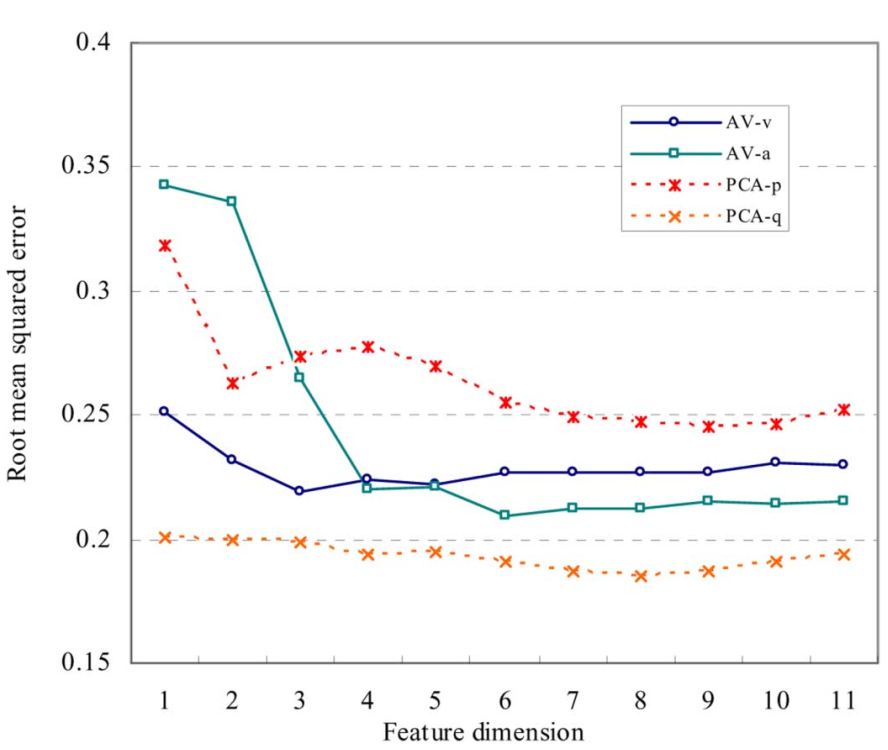
\includegraphics[width=0.48\textwidth, height=0.40\textwidth]{fig4.png}
\caption{Comparison of the root mean squared error using different feature dimensions for AV and PC. The features are the top ones selected by RReliefF.}
\label{fig3}
\end{figure}
\vspace{.5cm}


\bgroup
\def\arraystretch{1.4}
\begin{table}[ht]
    \centering
        \caption{TOP FIVE SELECTED FEATURES BY RRELIEFF FOR AV AND PC DATA SPACES}
        \label{table6}
    
    \begin{tabular}{ccc|ccc}
    \hline
\multicolumn{3}{c}{Arousal}       & \multicolumn{3}{c}{Valance}          \\ \hline
Name         & Extractor & weight & Name             & Extractor & weight \\ \hline
stdFlux      & M         & 0.0123 & spectral diss(S) & P*        & 0.0223 \\
tonality     & P*        & 0.0115 & tonality         & P*        & 0.0210 \\
multiplicity & P*        & 0.0095 & sum of bit hist  & M         & 0.0167 \\
meanFlux     & M         & 0.0093 & chord            & P*        & 0.0129 \\
meanRolloff  & M         & 0.0092 & sum of pitch     & M         & 0.0108\\ \hline \hline
 \multicolumn{6}{r}{*Psy15 features.}
\end{tabular}
\end{table}
\vspace{.5cm}

\begin{table}[ht]
    \centering
        \caption{$R^2$ STATISTICS FOR DIFFERENT COMBINATION OF DIFFERENT METHODS,
DATA SPACES, AND FEATURE SPACES}
        \label{table7}
    
    \begin{tabular}{ccccc}
    \hline
Method      & Data space & feature space & \multicolumn{2}{c}{\begin{tabular}[c]{@{}c@{}}$R^2$ statistics\\ a           v\end{tabular}} \\ \hline
MLR         & AV         & Psy15         & 56.8\%                                   & 10.9\%                                  \\
BoostR      & AV         & Psy15         & 55.3\%                                   & 11.7\%                                  \\
SVR         & AV         & Psy15         & 57.0\%                                   & 22.2\%                                  \\
SVR         & PC         & RRF$_{18,15}$           & 58.3\%                                   & 28.1\%                                  \\
Test-retest$^1$ & N/A        & N/A           & 80.5\%                                   & 58.6\%                                \\        \hline \hline
\multicolumn{5}{r}{$^1$The upper bound estimated in section V.$A$.}

\end{tabular}
\end{table}
\egroup
Results
shown in the first three rows of Table VII indicates that the $R$ of SVR reaches 57.0\% for arousal and 22.2\% for valence, representing the most prominent prediction accuracy among the three, and BoostR exhibits prediction accuracy similar to the baseline method MLR. Consequently, we employ SVR as the regressor in the following experiments.



\bgroup
\def\arraystretch{1}
\begin{table}[ht]
    \centering
        \caption{$R^2$ STATISTICS OF SVR WITH DIFFERENT DATA AND FEATURE SPACES}
        \label{table3}

\begin{tabular}{llll}
\hline
   & \multicolumn{1}{c}{\begin{tabular}[c]{@{}c@{}}ALL\\ a \ \ \ \ \ \ \ \ v\end{tabular}} & \multicolumn{1}{c}{\begin{tabular}[c]{@{}c@{}}Psy15\\ a \ \ \ \ \ \ \ \ v\end{tabular}} & \multicolumn{1}{c}{\begin{tabular}[c]{@{}c@{}}RRF\\ a \ \ \ \ \ \ \ \ v\end{tabular}} \\ \hline
AV & 58.6\%  \ \ \ \  14.6\%                                                               & 57.0\%  \ \ \ \  22.2\%                                                                 & 60.9\%  \ \ \ \  25.4\%                                                               \\ 
PC & 60.2\%  \ \ \ \  16.2\%                                                               & 58.5\%  \ \ \ \  18.1\%                                                                 & 58.3\%  \ \ \ \  28.1\%                                                               \\ \hline
\end{tabular}

\end{table}

\egroup

\subsection{Performance Evaluation of Data Space and Feature Space}
Next, we compare the $R^2$ of various combinations of data
spaces and feature spaces using SVR as the regressor. Result
shown in Table VIII indicates the following.
\begin{enumerate}
    \item The best combination of data and feature space by summing the $R^2$ of arousal and valence directly is PC + RRF$_{18,15}$, and the resulting $R^2$ reaches 58.3\% for arousal and 28.1\% for valence.

    \item Transforming the data to PC does not make significant difference to the prediction accuracy. This is interesting, since reducing the correlation between arousal and valence seems to have little influence. One possible reason to this phenomenon is that subjects can independently annotatearousal and valence to a certain extent, but it remains to validate this argument more rigorously.
    
    \item Selecting features by RRF greatly improves the accuracy (especially for valence), which shows the importance of feature selection. Generally the performance of adopted feature spaces is RRF $>$ Psy15 $>$ ALL.
    
    \item Using Psy15 as the feature space rather than ALL does not exhibit evident accuracy improvement for PC, which may be reasonable because the psychoacoustic meaning of the Psy15 features might be lost in the principal space.
    
    \item  Recall when we use AV + RRF, only three features are used to predict valence (see Table V); however, the reported $R^2$ 25.4\% is high enough compared to the best one 28.1\%. This finding implies most of the 114 extracted features may not be so relevant to valence.
\end{enumerate}

We also show the distributions of ground truth and prediction result for PC $+$ RRF$_{18,15}$ $+$ SVR in Fig. 5. It can be observed that the aggregated distributions are quite similar. Fig. 6 is obtained from in Fig. 5 by connecting predicted values to the corresponding ground truth values with lines.

In summary, the best performance of the regression approach reaches 58.3\% for arousal and 28.1\% for valence by using PC $+$ RRF$_{18,15}$ $+$ SVR. This performance is considered satisfactory since it meets over half the upper bound estimated from the testretest reliability study with less than 20 features for both arousal and valence (see the last two rows of Table VII).

To the best of our knowledge, there has been little previous work viewing MER from a continuous perspective. Therefore, in Section V-F we apply the regression approach to MEVD and compare our performance against the system ID approach [10], which has reported quantitative performance analysis and made dataset publicly available.

\subsection{ Performance Evaluation for MEVD}
To have a fair comparison, we apply the regression approach to MEVD by using the same ground truth data and feature data described in [10], where six classical music selections are segmented every second, and 18 musical features are extracted (17

\begin{figure}[h]
\centering
\captionsetup{justification=centering}
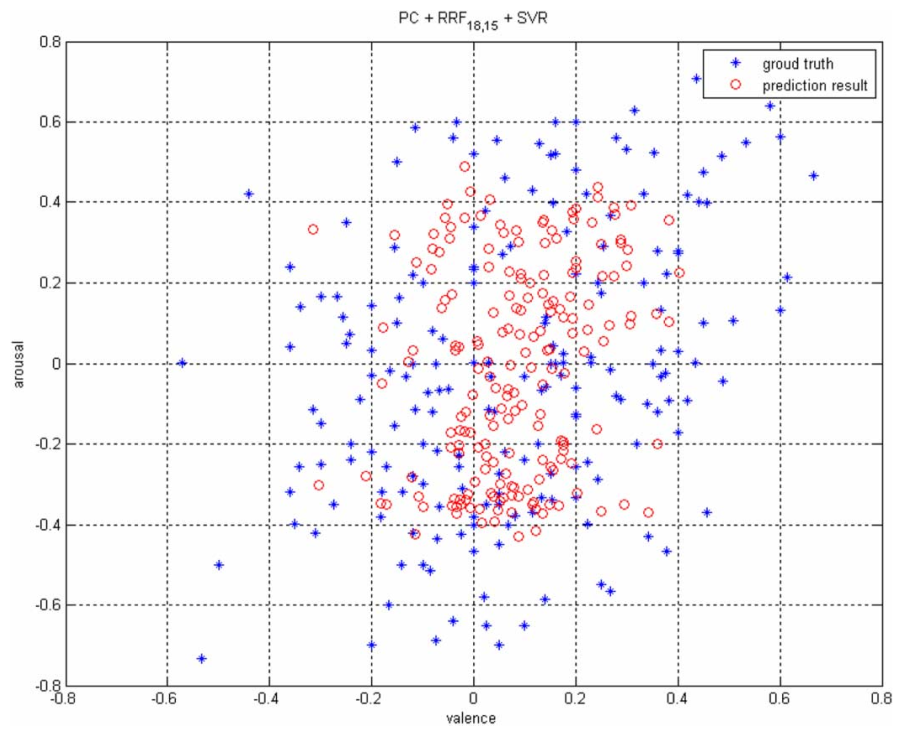
\includegraphics[width=0.48\textwidth, height=0.3\textwidth]{fig5.png}
\caption{Distributions of ground truth (blue point) and prediction result (red
circle) for PC + RRF$_{18,15}$ + SVR. It can be observed that the distributions
are similar. For a closer look, see Fig. 6}
\label{fig3}
\end{figure}

\begin{figure}[h]
\centering
\captionsetup{justification=centering}
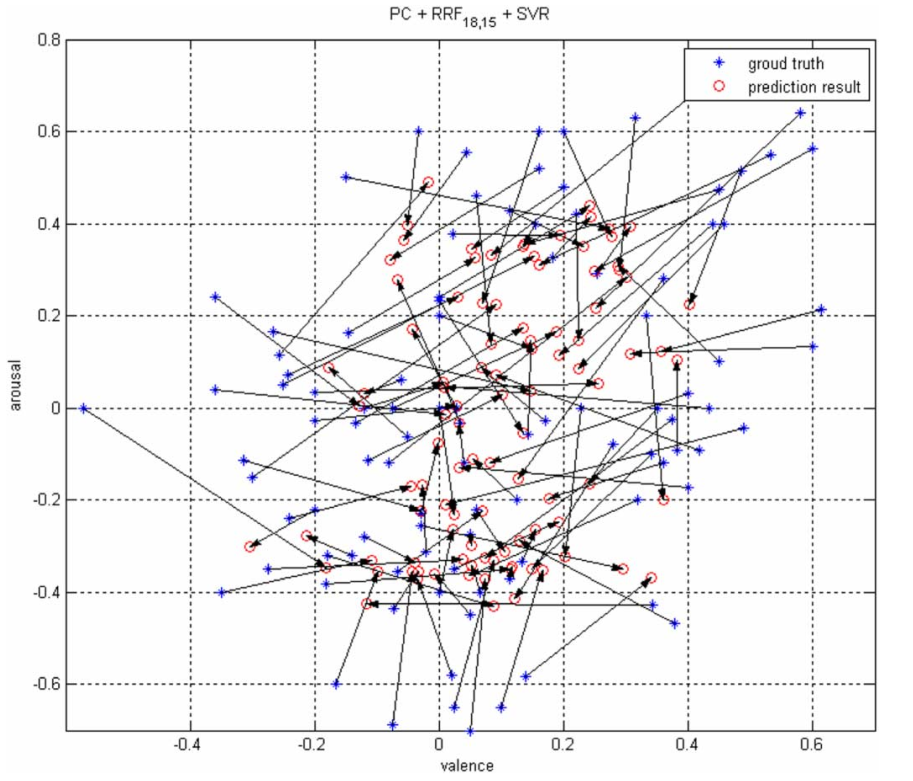
\includegraphics[width=0.48\textwidth, height=0.4\textwidth]{fig6.png}
\caption{Distributions of ground truth values (blue stars) with lines connecting
to the corresponding predicted values (red circles) by PC + RRF$_{18,15}$ + SVR
For space limitation, only 100 songs are shown.}
\label{fig3}
\end{figure}


\bgroup
\def\arraystretch{1.3}
\begin{table}[ht]
    \centering
        \caption{$R^2$ STATISTICS FOR MEVD USING THE SAME DATA AS [10]}
        \label{table7}
    \begin{tabular}{cccc}
\hline
Method                                              & Data                                                                                    & feature                                                                                              & \begin{tabular}[c]{@{}c@{}}$R^2$ statistics\\ a \ \ \ \ v\end{tabular} \\ \hline
\begin{tabular}[c]{@{}c@{}}System\\ ID\end{tabular} & \begin{tabular}[c]{@{}c@{}}6 classical music\\ annotated in the\\ AV space\end{tabular} & \begin{tabular}[c]{@{}c@{}}11PsySound features\\ +6 Marsyas features\\ +beat per minute\end{tabular} & 78.4\%  21.9\%                                             \\ 
SVR                                                 & As above                                                                                & As above                                                                                             & 64.8\%  52.9\%                                             \\ \hline
\end{tabular}
\end{table}
\egroup

of them are extracted by PsySound and Marsyas). The $R^2$ reported in \cite{10} is 78.4\% for arousal and 21.9\% for valence. We use SVR to predict the AV values for each 1-s segment and compute the average $R^2$ statistics. Results (64.8\% for arousal and 52.9\% for valence) shown in Table IX indicates the regression approach outperforms the system ID approach in a great extent for valence prediction and achieves comparable result for arousal prediction. This performance is remarkably good since the regression approach does not exploit any temporal information embedded in the time sequence. This experiment demonstrates the effectiveness of the regression approach for AV computation and shows the regression approach can be applied on
MEVD as well.

\section{DISCUSSION ON THE SUBJECTIVITY ISSUE}
The paper has focused on solving the ambiguity issue. In this
section, we discuss the ability of the regression approach to deal
with the subjectivity issue.

The subjectivity issue stems from the fact that music perception is intrinsically subjective and is under the influence of many factors such as cultural background, generation, sex, and personality. Therefore, as pointed out in [8], typical categorical approaches that simply assigning one emotion class to each song in a deterministic manner does not perform well in practice. Since the regression approach represents each song as a point in the emotion plane and thus offers more freedom in describing emotion, the prediction result is less deterministic. Besides the quadrant to which the song belongs, one can further know the
emotion intensity by inspecting the AV values. This result is obviously more reasonable and informative.

Despite that it has more freedom in describing a song, the regression approach may fail to exactly resolve the subjectivity issue since personal difference in the perception of popular music is too high, and since the regressors are trained based upon the average opinions of the subjects. It remains needed to address the subjectivity issue more effectively.

We develop a group-wise MER scheme (GWMER) to resolve this issue. The main idea is to divide the users into a variety of user groups and train regressors for each group. The groups can be defined according to user information \cite{34}, \cite{35} such as generation, sex, occupation, personality, etc., to reduce the individual differences for each group. The training process is similar to what we describe in Section IV except that the subjects are specified according to the target user group. The number of necessary subjects grows proportionally with the number of defined groups. After a collection of regressors have been trained, we can choose the most suitable $R_A$ and $R_V$ to respond to each user according to his/her personal information. In this way, the effect of a great number of individual factors is eliminated. See Fig. 7 for the system diagram.

Personalization offers an alternative way to resolve the subjectivity issue. However, building a personalized MER system is difficult because emotion perception may be too subtle to be understood and described quantitatively. Another issue for the personalization is the extra user burden.

GWMER represents a compromise between the general MER system presented in this paper and a personalized one. It can alleviate the subjectivity issue without resorting to too much user burden. Further investigation is worthwhile.








\section{Conclusion}
In this paper, a music selection is quantified as a point in the arousal-valence emotion plane. This continuous view of

\begin{figure}[h]
\centering
\captionsetup{justification=centering}
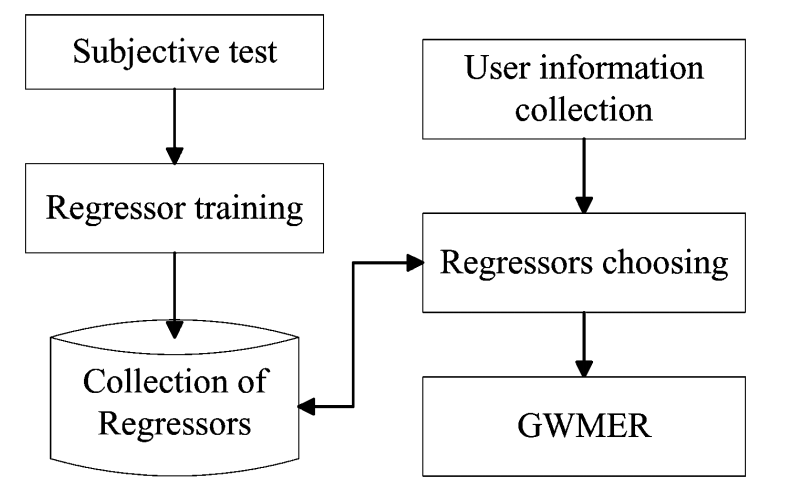
\includegraphics[width=0.35\textwidth, height=0.2\textwidth]{fig7.png}
\caption{GWMER scheme. A number of group-wise regressors are trained based
on the user opinions of different homogeneous user groups. Because the individual difference is reduced by grouping users, the subjectivity problem is believed to be alleviated. When a new user comes to use the MER system, his/her
user information is first collected, and then the appropriate $R_A$ and $R_V$ are
chosen to respond to the user.}
\label{fig3}
\end{figure}

music emotion makes the proposed MER system free of the inherent ambiguity issue from which conventional categorical approaches suffer. In addition, because there is more freedom in describing a song, the subjectivity issue is alleviated to some extent.

The accuracy of the AV computation determines the viability of the MER system. We formulate MER as a regression problem and adopt the support vector regression for direct estimation of the AV values. Comparing to existing AV computation algorithms, the regression approach has a sound theoretical foundation, exhibits promising prediction accuracy, and needs no temporal information or geometric operations.

Through an extensive performance study on the selection of data space, feature space, and regressor, we have demonstrated the effectiveness of the regression approach. The $R^2$ statistics reaches 58.3\% for arousal and 28.1\% for valence. We have also shown that the regression approach can be applied to MEVD and that it outperforms the approach proposed in \cite{10}.

Since arousal and valence may be dependent, we apply principal component analysis on the ground truth data to reduce the data correlation. The resulting little accuracy improvement implies the subjects can label arousal and valence quite independently. We also employ RReliefF to select features and find the accuracy greatly improved.

Future work will focus on exploiting features about lyrics and singing of a song, evaluating the regression approach on a largescale database, and realizing the GWMER scheme to further address the subjectivity issue.




% An example of a 3loating figure using the graphicx package.
% Note that \label must occur AFTER (or within) \caption.
% For figures, \caption should occur after the \includegraphics.
% Note that IEEEtran v1.7 and later has special internal code that
% is designed to preserve the operation of \label within \caption
% even when the captionsoff option is in effect. However, because
% of issues like this, it may be the safest practice to put all your
% \label just after \caption rather than within \caption{}.
%
% Reminder: the "draftcls" or "draftclsnofoot", not "draft", class
% option should be used if it is desired that the figures are to be
% displayed while in draft mode.
%
%\begin{figure}[!t]
%\centering
%\includegraphics[width=2.5in]{myfigure}
% where an .eps filename suffix will be assumed under latex, 
% and a .pdf suffix will be assumed for pdflatex; or what has been declared
% via \DeclareGraphicsExtensions.
%\caption{Simulation results for the network.}
%\label{fig_sim}
%\end{figure}

% Note that the IEEE typically puts floats only at the top, even when this
% results in a large percentage of a column being occupied by floats.


% An example of a double column floating figure using two subfigures.
% (The subfig.sty package must be loaded for this to work.)
% The subfigure \label commands are set within each subfloat command,
% and the \label for the overall figure must come after \caption.
% \hfil is used as a separator to get equal spacing.
% Watch out that the combined width of all the subfigures on a 
% line do not exceed the text width or a line break will occur.
%
%\begin{figure*}[!t]
%\centering
%\subfloat[Case I]{\includegraphics[width=2.5in]{box}%
%\label{fig_first_case}}
%\hfil
%\subfloat[Case II]{\includegraphics[width=2.5in]{box}%
%\label{fig_second_case}}
%\caption{Simulation results for the network.}
%\label{fig_sim}
%\end{figure*}
%
% Note that often IEEE papers with subfigures do not employ subfigure
% captions (using the optional argument to \subfloat[]), but instead will
% reference/describe all of them (a), (b), etc., within the main caption.
% Be aware that for subfig.sty to generate the (a), (b), etc., subfigure
% labels, the optional argument to \subfloat must be present. If a
% subcaption is not desired, just leave its contents blank,
% e.g., \subfloat[].


% An example of a floating table. Note that, for IEEE style tables, the
% \caption command should come BEFORE the table and, given that table
% captions serve much like titles, are usually capitalized except for words
% such as a, an, and, as, at, but, by, for, in, nor, of, on, or, the, to
% and up, which are usually not capitalized unless they are the first or
% last word of the caption. Table text will default to \footnotesize as
% the IEEE normally uses this smaller font for tables.
% The \label must come after \caption as always.
%
%\begin{table}[!t]
%% increase table row spacing, adjust to taste
%\renewcommand{\arraystretch}{1.3}
% if using array.sty, it might be a good idea to tweak the value of
% \extrarowheight as needed to properly center the text within the cells
%\caption{An Example of a Table}
%\label{table_example}
%\centering
%% Some packages, such as MDW tools, offer better commands for making tables
%% than the plain LaTeX2e tabular which is used here.
%\begin{tabular}{|c||c|}
%\hline
%One & Two\\
%\hline
%Three & Four\\
%\hline
%\end{tabular}
%\end{table}


% Note that the IEEE does not put floats in the very first column
% - or typically anywhere on the first page for that matter. Also,
% in-text middle ("here") positioning is typically not used, but it
% is allowed and encouraged for Computer Society conferences (but
% not Computer Society journals). Most IEEE journals/conferences use
% top floats exclusively. 
% Note that, LaTeX2e, unlike IEEE journals/conferences, places
% footnotes above bottom floats. This can be corrected via the
% \fnbelowfloat command of the stfloats package.









% if have a single appendix:
%\appendix[Proof of the Zonklar Equations]
% or
%\appendix  % for no appendix heading
% do not use \section anymore after \appendix, only \section*
% is possibly needed

% use appendices with more than one appendix
% then use \section to start each appendix
% you must declare a \section before using any
% \subsection or using \label (\appendices by itself
% starts a section numbered zero.)
%



% use section* for acknowledgment
\section*{Acknowledgment}
The authors would like to thank the reviewers for valuable
comments that greatly improved the quality of this paper.


% Can use something like this to put references on a page
% by themselves when using endfloat and the captionsoff option.
\ifCLASSOPTIONcaptionsoff
  \newpage
\fi



% trigger a \newpage just before the given reference
% number - used to balance the columns on the last page
% adjust value as needed - may need to be readjusted if
% the document is modified later
%\IEEEtriggeratref{8}
% The "triggered" command can be changed if desired:
%\IEEEtriggercmd{\enlargethispage{-5in}}

% references section

% can use a bibliography generated by BibTeX as a .bbl file
% BibTeX documentation can be easily obtained at:
% http://mirror.ctan.org/biblio/bibtex/contrib/doc/
% The IEEEtran BibTeX style support page is at:
% http://www.michaelshell.org/tex/ieeetran/bibtex/
%\bibliographystyle{IEEEtran}
% argument is your BibTeX string definitions and bibliography database(s)
%\bibliography{IEEEabrv,../bib/paper}
%
% <OR> manually copy in the resultant .bbl file
% set second argument of \begin to the number of references
% (used to reserve space for the reference number labels box)
\begin{thebibliography}{1}

\bibitem{1}
Y.~Feng, Y.~Zhuang, and Y.~Pan, “Popular music retrieval by detecting
mood,” Proc. ACM SIGIR, pp. 375–376, 2003.

\bibitem{2}
T. Li and M. Ogihara, “Content-based music similarity search and emotion detection,” in Proc. Int. Conf. Acoust., Speech, Signal Process.,
Toulouse, France, 2006, pp. 17–21.

\bibitem{3}
L. Lu, D. Liu, and H.-J. Zhang, “Automatic mood detection and
tracking of music audio signals,” IEEE Trans. Audio, Speech, Lang.
Process., vol. 14, no. 1, pp. 5–18, Jan. 2006.

\bibitem{4}
 M.-Y. Wang, N.-Y. Zhang, and H.-C. Zhu, “User-adaptive music
emotion recognition,” in Proc. Int. Conf. Sig. Process., 2004, pp.
1352–1355.

\bibitem{5}
T.-L. Wu and S.-K. Jeng, “Extraction of segments of significant emotional expressions in music,” in Proc. Int. Workshop Comput. Music
Audio Technol., 2006, pp. 76–80.


\bibitem{6}
D. Yang and W. Lee, “Disambiguating music emotion using software
agents,” in Proc. Int. Conf. Music Inf. Retrieval, 2004, pp. 52–58.


\bibitem{7}
V. Carvalho and C. Chao, “Sentiment retrieval in popular music based
on sequential learning,” Proc. ACM SIGIR, 2005 [Online]. Available:
http://www.mit.edu/~chihyu/projects/carvalho\_chao\_sigir05.pdf



\bibitem{8}
Y.-H. Yang, C.-C. Liu, and H. H. Chen, “Music emotion classification: A fuzzy approach,” in Proc. ACM Multimedia, Santa Barbara, CA,
2006, pp. 81–84.



\bibitem{9}
A. Hanjalic and L.-Q. Xu, “Affective video content representation and
modeling,” IEEE Trans. Multimedia, vol. 7, no. 1, pp. 143–154, Feb.
2005.


\bibitem{10}
M. D. Korhonen, D. A. Clausi, and M. E. Jernigan, “Modeling emotional content of music using system identification,” IEEE Trans. Syst.,
Man., Cybern., vol. 36, no. 3, pp. 588–599, Jun. 2006.

\bibitem{11}
E. Schubert, “Measurement and time series analysis of emotion in
music,” Ph.D. dissertation, School of Music Music Education, Univ.
New South Wales, Sydney, NSW, Australia, 1999.


\bibitem{12}
R. E. Thayer, The Biopsychology of Mood and Arousal. New York:
Oxford Univ. Press, 1989.


\bibitem{13}
P. J. Lang, “The emotion probe,” Amer. Psychol., vol. 50, no. 5, pp.
372–385, 1995.


\bibitem{14}
J. A. Russell, A. Weiss, and G. A. Mendelsohn, “Affect grid: A singleitem scale of pleasure and arousal,” J. Personality Social Psychol., vol.
57, no. 3, pp. 493–502, 1989.


\bibitem{15}
R. Cowie, E. Douglas-Cowie, S. Savvidou, E. McMahon, M. Sawey,
and M. Schröder, “’FEELTRACE’: An instrument for recording perceived emotion in real time,” in Proc. Speech Emotion, ISCA Tutorial
Res. Workshop, Newcastle, U.K., 2000, pp. 19–24.


\bibitem{16}
R. O. Duda, P. E. Hart, and D. G. Stork, Pattern Recognition. New
York: Wiley, 2000.


\bibitem{17}
A. Sen and M. Srivastava, Regression Analysis: Theory, Methods, and
Applications. New York: Springer, 1990.


\bibitem{18}
A. J. Smola and B. Schölkopf, “A tutorial on support vector regression,”
Statist. Comput., pp. 199–222, 2004.


\bibitem{19}
 C.-C. Chang and C.-J. Lin, LIBSVM: A library for support vector machines 2001 [Online]. Available: http://www.csie.ntu.edu.tw/sim cjlin/
libsvm


\bibitem{20}
D. P. Solomatine and D. L. Shrestha, “AdaBoost.RT: A boosting algorithm for regression problems,” in Proc. IEEE Int. Joint Conf. Neural
Netw., 2004, pp. 1163–1168.


\bibitem{21}
P. Viola and M. J. Jones, “Robust real-time face detection,” Int. J.
Comput. Vision, vol. 57, no. 2, pp. 137–154, 2004.


\bibitem{22}
M. R. Sikonja and I. Kononenko, ˇ “Theoretical and empirical analysis
of relieff and RRelieFF,” Mach. Learn. J., vol. 53, pp. 23–69, 2003.


\bibitem{23}
L. C. Molina, L. Belanche, and A. Nebot, “Feature selection algorithms: A survey and experimental evaluation,” in Proc. IEEE Int. Conf.
Data Mining, 2002, pp. 306–313.


\bibitem{24}
J. M. Keller, M. R. Gray, and J. A. Givens, “Fuzzy k-nearest neighbor
algorithm,” IEEE Trans. Syst., Man, Cybern., vol. SMC-15, no. 4, pp.
580–584, Aug. 1985.


\bibitem{25}
D. Tran, M. Wagner, and T. Zheng, “Fuzzy nearest prototype classifier
applied to speaker identification,” Proc. ESIT, 1999 [Online]. Available: http://www.erudit.de/erudit/events/esit99/12615\_p.pdf


\bibitem{26}
N. C. Maddage, C. Xu, M. S. Kankanhalli, and X. Shao, “Contentbased music structure analysis with applications to music semantics
understanding,” in Proc. ACM Multimedia, 2004, pp. 112–119.


\bibitem{27}
D. Cabrera, “PSYSOUND: A computer program for psychoacoustical
analysis,” in Proc. Australian Acoust. Soc. Conf., 1999, pp. 47–54 [Online]. Available: http://www.psysound.org


\bibitem{28}
J. Ricard, “Towards computational morphological description of
sound,” Ph.D. dissertation, Univ. Pompeu Fabra, Barcelona, Spain,
2004.



\bibitem{29}
G. Tzanetakis and P. Cook, “Musical genre classification of audio signals,” IEEE Trans. Speech Audio Process., vol. 10, no. 5, pp. 293–302,
Jul. 2002.


\bibitem{30}
A. Meng, P. Ahrendt, J. Larsen, and L. K. Hansen, “Temporal feature
integration for music genre classification,” IEEE Trans. Audio, Speech,
Lang. Process., vol. 15, no. 5, pp. 1654–1663, Jul. 2007.



\bibitem{31}
“Musicovery:Interactive Webradio.” [Online]. Available: http://www.
musicovery.com/


\bibitem{32}
D. C. Montgomery, G. C. Runger, and N. F. Hubele, Engineering Statistics. New York: Wiley, 1998.


\bibitem{33}
R. J. Cohen and M. Swerdlik, Psychological Testing and Measurement: An Introduction to Tests and Measurement. Mountain View,
CA: Mayfield, 1996.


\bibitem{34}
W. Chai and B. Vercoe, “Using user models in music information retrieval systems,” in Proc. Int. Symp. Music Inf. Retrieval, 2000 [Online]. Available: http://www.media.mit.edu/~chaiwei/papers/usermodeling.pdf



\bibitem{35}
M. Lesaffre, M. Leman, and J.-P. Martens, “A user-oriented approach
to music information retrieval,” in Content-Based Retrieval. Wadern,
Germany: Dagstuhl Seminar Proceedings, 2006.




%    \bibitem{IEEEhowto:kopka}
%   H.~Kopka and P.~W. Daly, \emph{A Guide to \LaTeX}, 3rd~ed.\hskip 1em plus
%     0.5em minus 0.4em\relax Harlow, England: Addison-Wesley, 1999.

\end{thebibliography}

% biography section
% 
% If you have an EPS/PDF photo (graphicx package needed) extra braces are
% needed around the contents of the optional argument to biography to prevent
% the LaTeX parser from getting confused when it sees the complicated
% \includegraphics command within an optional argument. (You could create
% your own custom macro containing the \includegraphics command to make things
% simpler here.)
%\begin{IEEEbiography}[{\includegraphics[width=1in,height=1.25in,clip,keepaspectratio]{mshell}}]{Michael Shell}
% or if you just want to reserve a space for a photo:

\begin{IEEEbiography}[{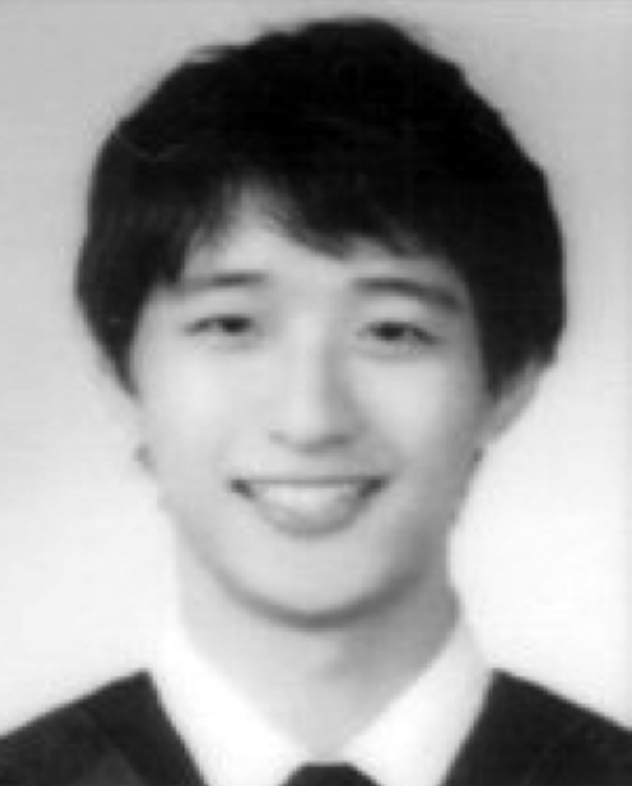
\includegraphics[width=1in,height=1.25in,clip,keepaspectratio]{fig8}}]{\bf Yi-Hsuan Yang}
received the B.S. degree in electrical engineering from National Taiwan University
(NTU), Taiwan, R.O.C., in 2006. He is currently
working toward the Ph.D. degree in the Graduate
Institute of Communication Engineering, NTU.
His research interests include multimedia information retrieval and analysis, human-centered
computing, and affective computing.
\end{IEEEbiography}

\begin{IEEEbiography}[{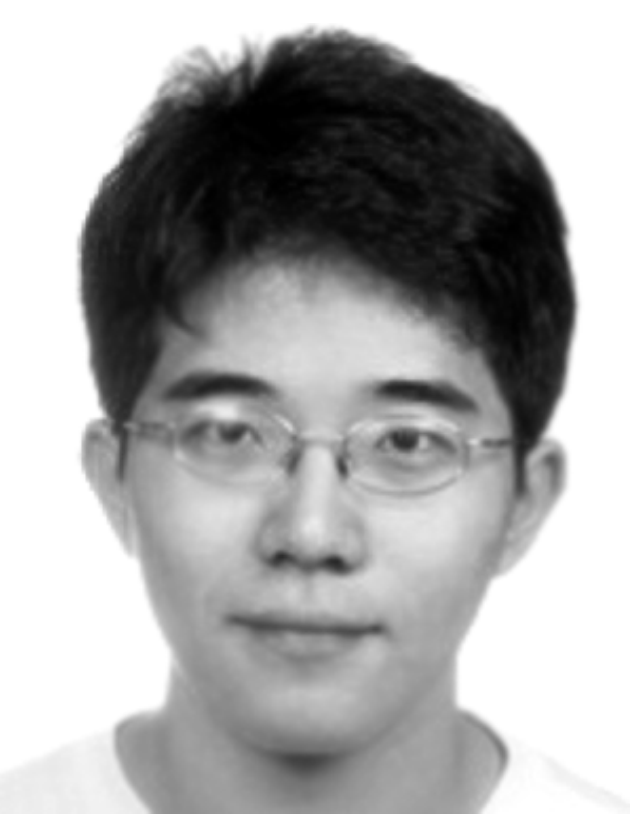
\includegraphics[width=1in,height=1.25in,clip,keepaspectratio]{fig9}}]{\bf Yu-Ching Lin}
received the B.S. degree in electrical engineering from National Taiwan University
(NTU), Taiwan, R.O.C., in 2007. He is currently
working toward the M.S. degree in the Graduate
Institute of Communication Engineering, NTU.
His research interests include music signal processing, machine learning, and affective computing.
\end{IEEEbiography}

\begin{IEEEbiography}[{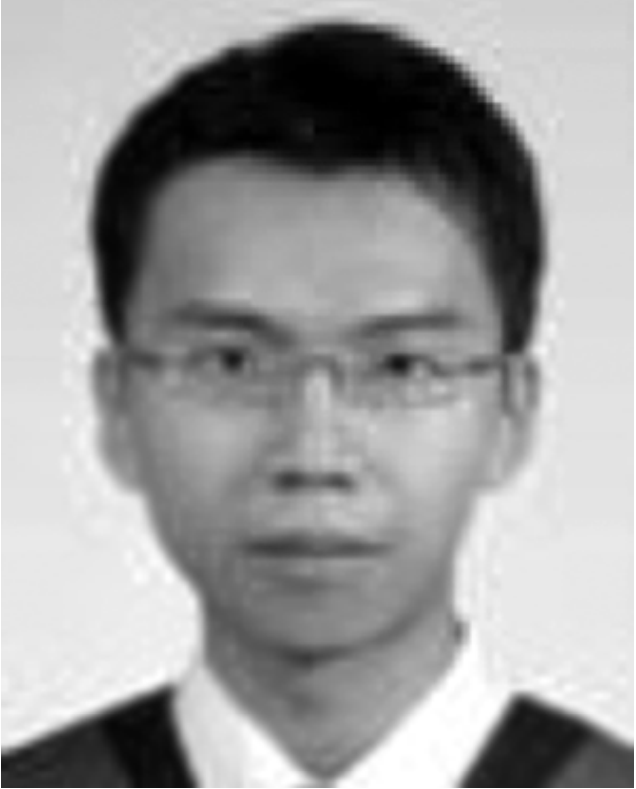
\includegraphics[width=1in,height=1.25in,clip,keepaspectratio]{fig10}}]{\bf Ya-Fan Su}
 received the B.S. degree in electrical engineering from National Taiwan University (NTU),
Taiwan, R.O.C., in 2007. He is currently working
toward the M.S. degree in the Graduate Institute of
Communication Engineering, NTU.
His research interests include video content
analysis, human-centered computing, and affective
computing.
\end{IEEEbiography}

\begin{IEEEbiography}[{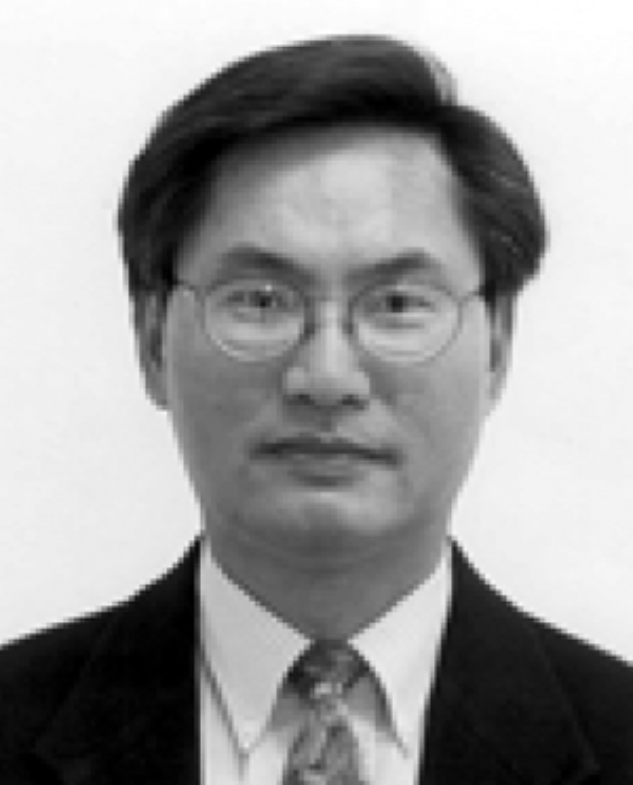
\includegraphics[width=1in,height=1.25in,clip,keepaspectratio]{fig11}}]{\bf Homer H. Chen}
(S’83–M’86–SM’01–F’03) received the Ph.D. degree in electrical and computer
engineering from the University of Illinois at
Urbana-Champaign.
Since August 2003, he has been with the College
of Electrical Engineering and Computer Science,
National Taiwan University, where he is the Irving T.
Ho Chair Professor. Prior to that, he had held various
R&D management and engineering positions in
U.S. companies over a period of 17 years, including
AT&T Bell Labs, Rockwell Science Center, iVast,
and Digital Island. He was a U.S. delegate for ISO and ITU standards committees and contributed to the development of many new interactive multimedia
technologies that are now part of the MPEG-4 and JPEG-2000 standards. His
professional interests lie in the broad area of multimedia signal processing and
communications.

Dr. Chen is an Associate Editor of the IEEE TRANSACTIONS ON CIRCUITS AND
SYSTEMS FOR VIDEO TECHNOLOGY. He served as Associate Editor for IEEE
TRANSACTIONS ON IMAGE PROCESSING from 1992 to 1994, Guest Editor for
IEEE TRANSACTIONS ON CIRCUITS AND SYSTEMS FOR VIDEO TECHNOLOGY in
1999, and Editorial Board Member for Pattern Recognition from 1989 to 1999.
\end{IEEEbiography}



% if you will not have a photo at all:


% insert where needed to balance the two columns on the last page with
% biographies
%\newpage

% You can push biographies down or up by placing
% a \vfill before or after them. The appropriate
% use of \vfill depends on what kind of text is
% on the last page and whether or not the columns
% are being equalized.

%\vfill

% Can be used to pull up biographies so that the bottom of the last one
% is flush with the other column.
%\enlargethispage{-5in}



% that's all folks
\end{document}

